\section{Introduction}
\begin{figure}[t]
  \centering
  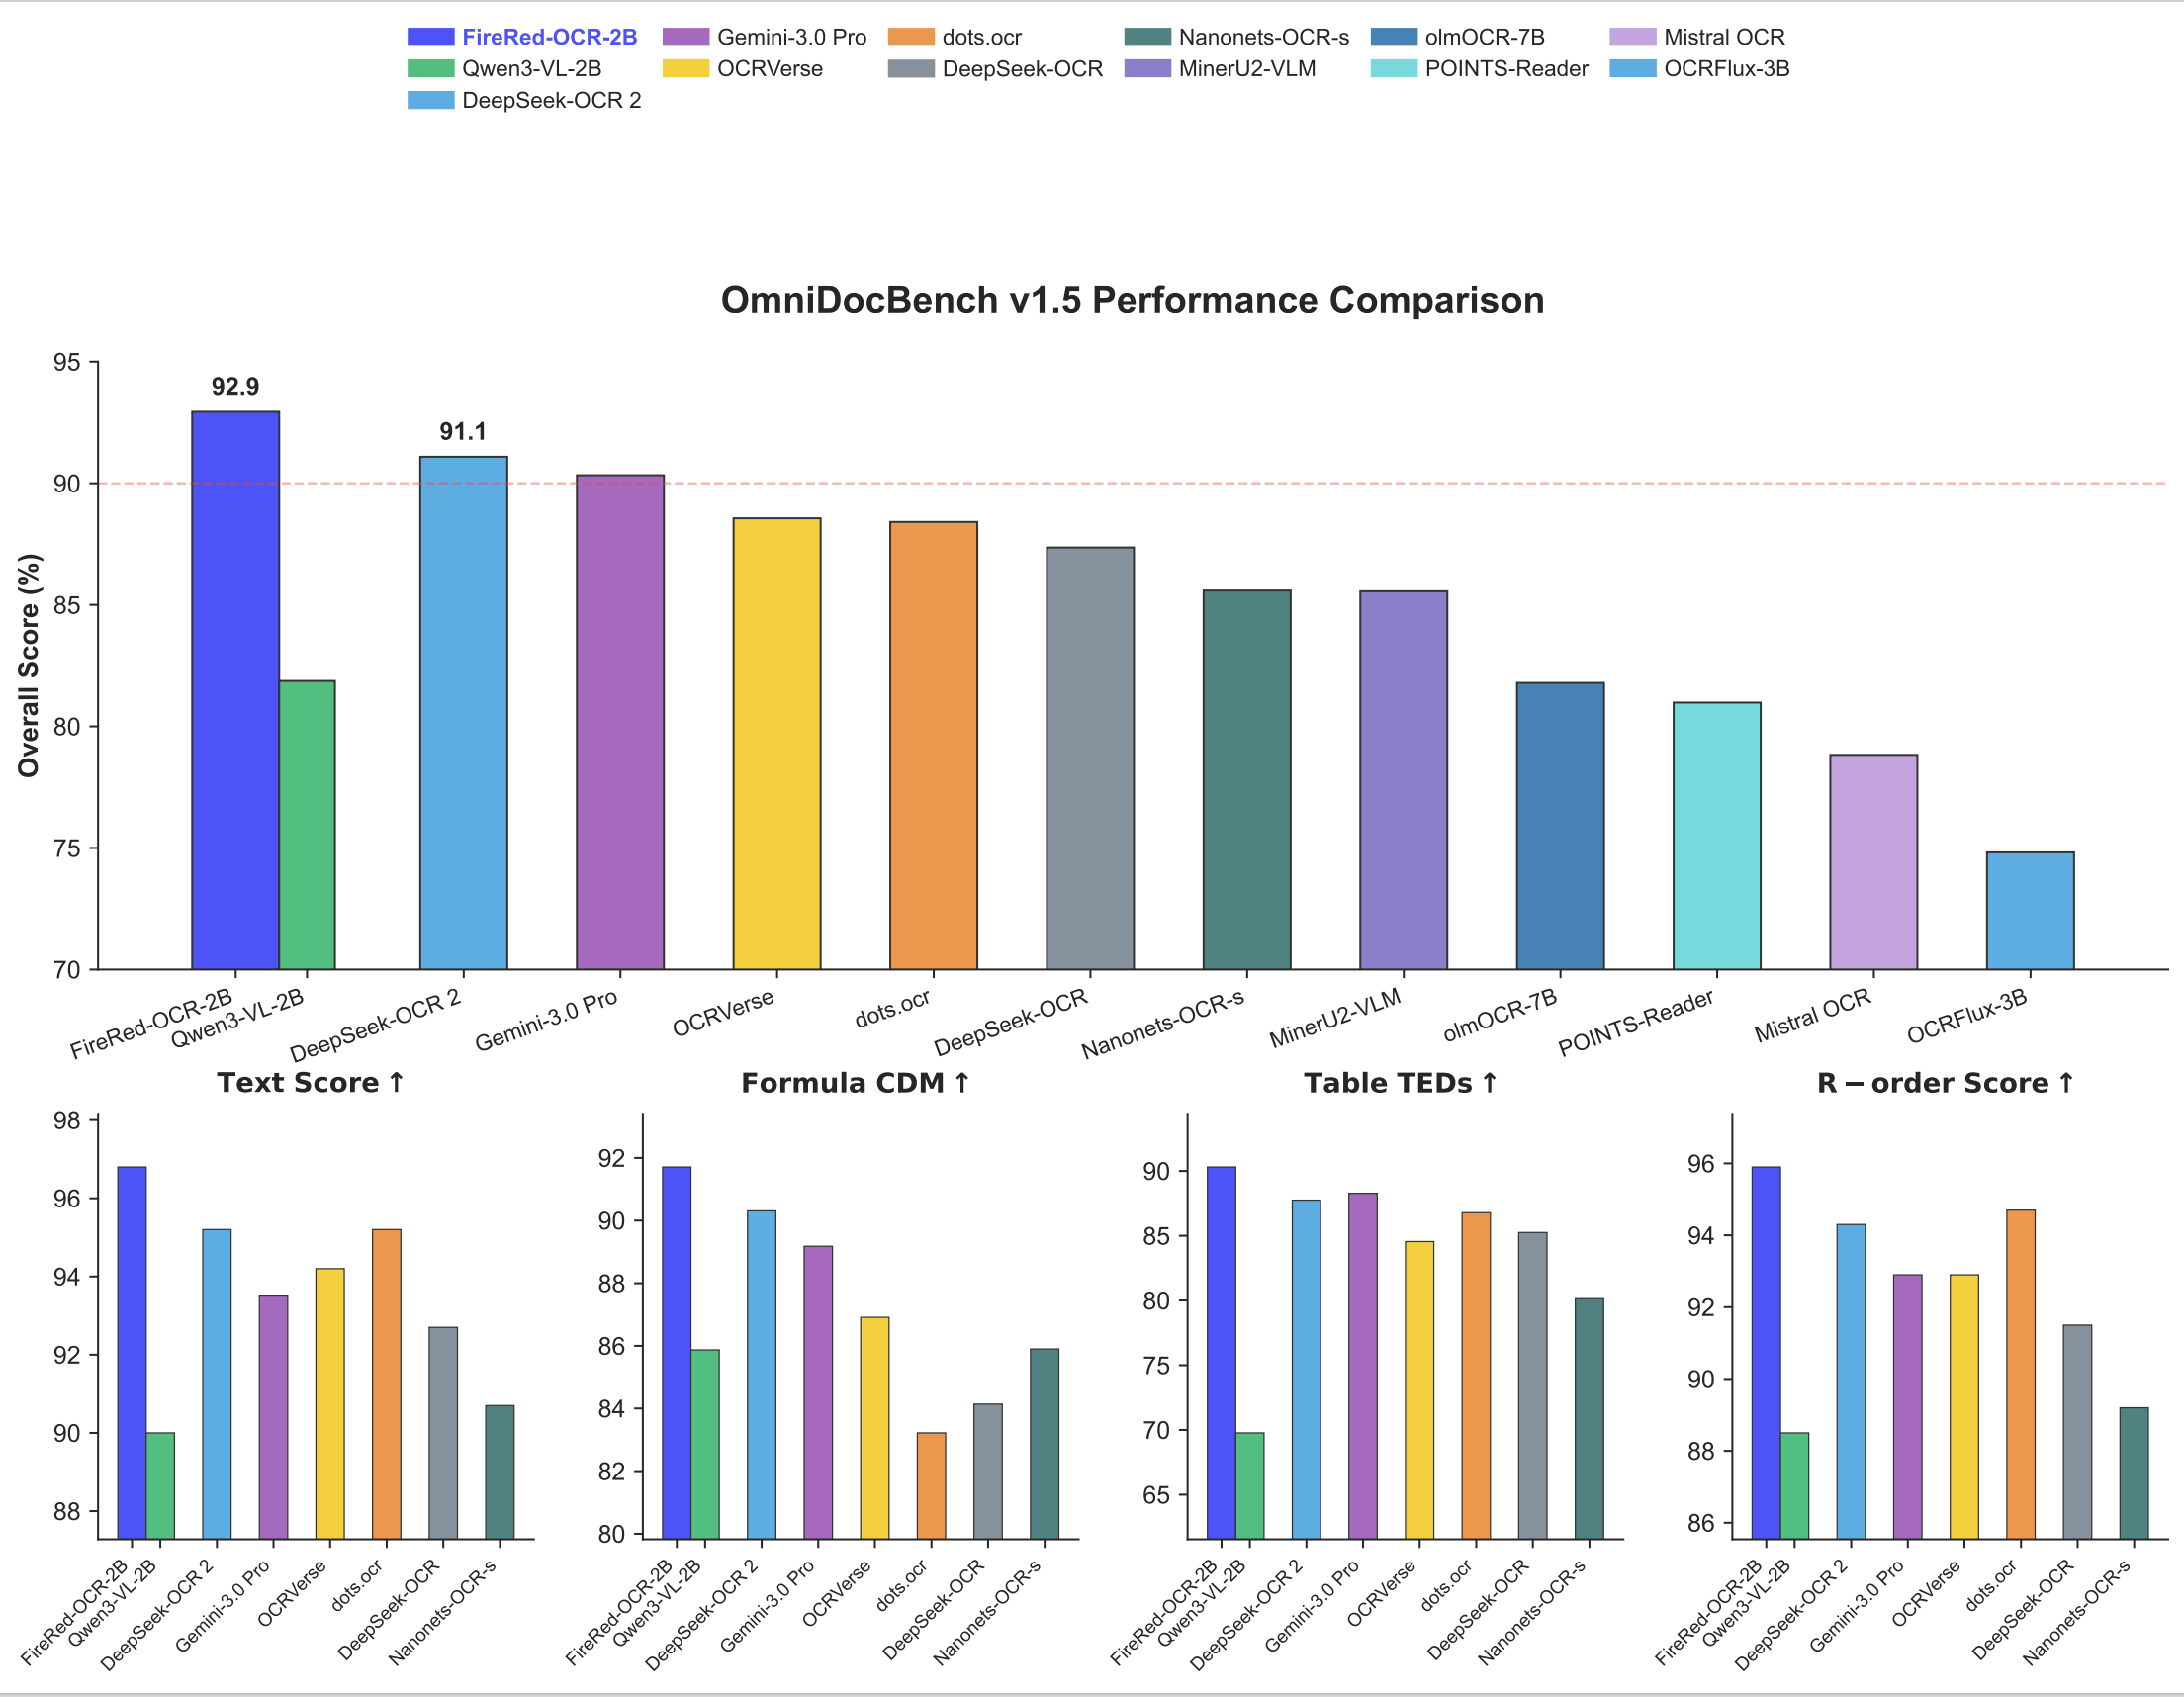
\includegraphics[width=0.99\textwidth]{figures/omnidoc_228.png}
  \caption{Comparison with state-of-the-art models on OmniDocBench v1.5~\cite{ouyang2025omnidocbench}. FireRed-OCR ranks first in the overall metric (top) and demonstrates leading performance across all sub-categories: Text recognition, Formula processing, Table structure analysis, and Reading order inference (bottom).}
  \label{fig:introduction_benchmark}
\end{figure}
The rapid evolution of Large Vision-Language Models (VLMs)~\cite{chen2023vlp,wang2024qwen2,chen2023x,zhang2024mm} has marked a transformative milestone in multimodal artificial intelligence~\cite{zhang2023structure,google2025gemini3pro}. Models such as GPT-4V~\cite{hurst2024gpt}, Qwen-VL~\cite{bai2023qwen}, and LLaVA~\cite{liu2023visual} have demonstrated remarkable capabilities in general image captioning and reasoning. However, these general-purpose models often exhibit significant instability when applied to Document Intelligence tasks involving the parsing of financial reports, academic papers, and complex forms. While they possess the semantic capacity to interpret visual content, they frequently fail to adhere to rigorous formatting constraints. We define this phenomenon as \textbf{Structural Hallucination}, which manifests as disordered rows in Markdown tables, non-existent syntax in mathematical formulas, or the omission of hierarchical logic. Such errors render the outputs effectively unusable for downstream industrial applications. The fundamental challenge, therefore, lies in transitioning the model's behavior from broad semantic interpretation to precise structural generation governed by strict logical rules.

Traditional OCR systems~\cite{cui2025paddleocr,cui2026paddleocr,zhang2025monkeyocr}, such as PaddleOCR-VL~\cite{cui2025paddleocr}, rely on pipeline approaches (detection followed by recognition). While pixel-precise, they often lack the semantic understanding required to reconstruct logical structures like reading order in multi-column layouts. Conversely, recent End-to-End approaches, including DeepSeek-OCR~\cite{wei2025deepseek}, DeepSeek-OCR 2~\cite{wei2026deepseek}, OCRVerse~\cite{zhong2026ocrverse}, and varying generic VLMs~\cite{bai2025qwen3,chen2025mindvl,team2023gemini,google2025gemini3pro}, treat document parsing as a sequence generation task. Although these models capture semantics better than traditional pipelines, they struggle with fine-grained spatial grounding. Existing general VLMs, despite their size, often lack the specialized alignment data and reinforcement mechanisms required to suppress hallucinations in dense text environments. They understand the ``intent'' but not the ``rules.''

To bridge this gap, we present \textbf{FireRed-OCR}, a framework designed to evolve a general VLM (specifically Qwen3-VL~\cite{bai2025qwen3}) into an industrial-grade structural expert. Our approach is founded on two pillars: a high-precision data engine and a progressive training strategy.

First, we address the data quality bottleneck by constructing a \textbf{``Geometry + Semantics'' Data Factory}. Traditional random sampling fails to capture the diversity of document layouts. We introduce a dual-indexing mechanism that clusters documents based on geometric features and semantic tags, enabling balanced sampling of rare layouts. We further implement an automated synthesis pipeline for scarce data and employ a ``Expert-Level Refinement'' process using advanced models to correct hard cases.

Second, we propose a \textbf{Three-Stage Progressive Training} pipeline to ``tame'' the model:
\begin{enumerate}
    \item \textbf{Multi-task Pre-alignment:} We force the model to learn physical perception (bounding boxes and region recognition) before attempting full-page generation.
    \item \textbf{Specialized SFT:} We refine the model on high-quality Markdown data to ensure standard syntax adherence.
    \item \textbf{Format-Constrained GRPO:} We introduce a Reinforcement Learning stage using Group Relative Policy Optimization (GRPO)~\cite{shao2024deepseekmath} with specific rewards for formula validity, table closure, and content accuracy, endowing the model with self-correction capabilities.
\end{enumerate}

Our contributions are summarized as follows:
\begin{itemize}
    \item We identify \textit{Structural Hallucination} as the primary bottleneck in VLM-based document parsing and propose a solution that shifts the paradigm from text generation to structural engineering.
    \item We develop a ``Geometry + Semantics'' Data Factory that ensures interpretable, balanced, and high-quality supervision data.
    \item We introduce a three-stage training strategy incorporating constrained GRPO, significantly improving robustness in complex layout reconstruction.
    \item FireRed-OCR achieves SOTA results on the authoritative \textbf{OmniDocBench v1.5}, surpassing DeepSeek-OCR2 and OCRVerse with a 92.94\% overall score, proving the viability of our ``General VLM $\rightarrow$ Specialized Structural Model'' paradigm.
\end{itemize}